%%
%% This is file 'sample-degree-report.tex' was based on the ACM's`sample-manuscript.tex'.
%% Note that this was taken from the Overleaf project: https://www.overleaf.com/gallery/tagged/acm-official#.WOuOk2e1taQ
%% It has been adapted to use the TIMTM template (adapted from CHI Proceedings Template) for
%% the Interactive Media Technology (TIMTM) and Media Management (TMMTM) programmes at KTH Royal Institute of Technology.
%% 
%% 2021-11-09 Gerald Q. Maguire Jr. adapted template to KTH's TIMTM and TMMTM requirements, including:
%% removing the ACM copyright and other notices in the generate documents - as these are not applicable
%% and rewriting some of the contents of the sample document.
%% Note that the teaserfigure environment simply ignores content, s there should
%% note be teaser figures in a thesis.
%%§
%%
%% IMPORTANT NOTICE:
%% 
%% For the copyright see the file: acmart-primary/acmart.dtx - from the github
%%
%% The first command in your LaTeX source must be the \documentclass command.

%%%% Generic manuscript mode, required for submission
%%%% and peer review
%\documentclass[manuscript,screen,review]{timtm}
\documentclass[manuscript, screen]{timtm}
%% If you add the review option, then line numbers are added to the manuscript.
%% Note that as the thesis is in a single column format,
%%  the line numbers are only on the left.
%% The option authordraft adds a draft watermark.

%% Some of the options have been removed, as they did not make sense for a thesis.
%% Note that there is not an anonymous option, as theses are never anonymous.
%% There is also not authorversion option.
%% Note that you do not need the sigcconf for the thesis template

%% Fonts used in the template cannot be substituted; margin 
%% adjustments are not allowed.
%%
%% \BibTeX command to typeset BibTeX logo in the docs
\makeatletter%
\@ifclassloaded{acmart}%
  {\AtBeginDocument{%
  \providecommand\BibTeX{{%
   \normalfont B\kern-0.5em{\scshape i\kern-0.25em b}\kern-0.8em\TeX}}}}%
  {\AtBeginDocument{%
  \providecommand\BibTeX{{%
   \rm B\kern-.05em{\sc i\kern-.025em b}\kern-.08em\TeX}}}}%
\makeatother%



%% Note that it you do happen to repurpose this file for a submission to SIGCHI, you might add the line below - as you need to retain the copyright, since KTH must be able to distribute copies upon request.
\setcopyright{rightsretained}

\copyrightyear{2022}

%% For an actual ACM submission
%% Rights management information.  This information is sent to you
%% when you complete the rights form.  These commands have SAMPLE
%% values in them; it is your responsibility as an author to replace
%% the commands and values with those provided to you when you
%% complete the rights form.
%\setcopyright{acmcopyright}
%\copyrightyear{2018}
%\acmYear{2018}
%\acmDOI{10.1145/1122445.1122456}

%% These commands are for a PROCEEDINGS abstract or paper.
%\acmConference[Woodstock '18]{Woodstock '18: ACM Symposium on Neural  Gaze Detection}{June 03--05, 2018}{Woodstock, NY}
%\acmBooktitle{Woodstock '18: ACM Symposium on Neural Gaze Detection,  June 03--05, 2018, Woodstock, NY}
%\acmPrice{15.00}
%\acmISBN{978-1-4503-XXXX-X/18/06}


%%
%% Submission ID.
%% Use this when submitting an article to a sponsored event. You'll
%% receive a unique submission ID from the organizers
%% of the event, and this ID should be used as the parameter to this command.
%%\acmSubmissionID{123-A56-BU3}

%%
%% Use numbered citations and references. 
%%
% include a variety of packages that are useful
\input{lib/includes}
\input{lib/kthcolors}

%\input{lib/defines}  % load some additional definitions to make writing more consistent


%% If the acmart document class is being used, define away some commands and environment
%% If not, then enable ISBNs to be shown in references
\makeatletter%
\@ifclassloaded{acmart}%
{%
\newcommand{\alttitle}[1]{}
\newcommand{\altsubtitle}[1]{}
\newenvironment{swedishabstract}{}{}
\newcommand{\SwedishKeywords}[1]{}
}{%
% Define these so that the bibliography will include ISBNs
\newcommand{\showISBNx}{}
\newcommand{\showISBNxiii}{}
}%
\makeatother%


%% end of the preamble, start of the body of the document source.
\begin{document}
% insert the configuration information with author(s), examiner, supervisor(s), ...
\input{custom_configuration}

%%
%% The "title" command has an optional parameter,
%% allowing the author to define a "short title" to be used in page headers.
\title{The Report Title}
%\subtitle{A short subtitle}

% give the alternative title - i.e., if the thesis is in English, then give a Swedish title
\alttitle{Detta är den svenska översättningen av titeln}
\altsubtitle{Detta är den svenska översättningen av undertiteln}
\makeatletter

%%
%% The "author" command and its associated commands are used to define
%% the authors and their affiliations.
%% Of note is the shared affiliation of the first two authors, and the
%% "authornote" and "authornotemark" commands
%% used to denote shared contribution to the research.

%% For the thesis template we will take the authors names and e-mail addresses from the custom_configuration.tex file
\author{\@authorsFirstname\space\@authorsLastname}
%\authornote{Both authors contributed equally to this research.}
\email{\@email}
%\orcid{1234-5678-9012}
%% If there is no second author (which should be the case for a second cycle thesis
%% comment out the following line and the additional \email line
\author{\@secondAuthorsFirstname\space\@secondAuthorsLastname}
% Apply the same authornote for the second author
%\authornotemark[1]
\email{\@secondemail}
%\orcid{1234-5678-901X}
\affiliation{%
  \institution{KTH Royal Institute of Technology, School of Electrical Engineering and Computer Science}
  %\streetaddress{Street address}
  \city{Stockholm}
  \country{Sweden}
  \postcode{SE 100 44}
}
\makeatother

%%
%% The abstract is a short summary of the work to be presented in the
%% article.
\begin{abstract}
\begin{scontents}[store-env=abstracts,print-env=false]
  This sample report describes the formatting
  requirements for a Interactive Media Technology (TIMTM) and Media Management (TMMTM) programmes at KTH Royal Institute of Technology. It is based upon the ACM conference proceedings format, and offers
  recommendations on writing for the worldwide SIGCHI
  readership. Please review this document, as some format details have changed
  relative to previous years. Note that the template now generates the KTH front cover, titlepage, and information for entering the meta data associated with your thesis into DiVA. Abstracts should be about 150 words.
  
  All theses at KTH are \textit{required} to have an abstract in \textbf{both} English and Swedish.
 \end{scontents}
\end{abstract}

\begin{swedishabstract}
\begin{scontents}[store-env=abstracts,print-env=false]
Alla avhandlingar vid KTH \textit{måste ha} ett abstrakt på \textbf{både} engelska och svenska.

Om du skriver din avhandling på svenska ska detta göras först (och placera det som det första abstraktet) - och du bör revidera det vid behov. Om du gör detta måste du ändra dokumentmallen - eftersom den förutsätter att den första sammanfattningen är på engelska och den andra på svenska.
\end{scontents}
\end{swedishabstract}

%%
%% The code below is generated by the tool at http://dl.acm.org/ccs.cfm.
%% Please copy and paste the code instead of the example below.
%%
\begin{CCSXML}
<ccs2012>
 <concept>
  <concept_id>10010520.10010553.10010562</concept_id>
  <concept_desc>Computer systems organization~Embedded systems</concept_desc>
  <concept_significance>500</concept_significance>
 </concept>
 <concept>
  <concept_id>10010520.10010575.10010755</concept_id>
  <concept_desc>Computer systems organization~Redundancy</concept_desc>
  <concept_significance>300</concept_significance>
 </concept>
 <concept>
  <concept_id>10010520.10010553.10010554</concept_id>
  <concept_desc>Computer systems organization~Robotics</concept_desc>
  <concept_significance>100</concept_significance>
 </concept>
 <concept>
  <concept_id>10003033.10003083.10003095</concept_id>
  <concept_desc>Networks~Network reliability</concept_desc>
  <concept_significance>100</concept_significance>
 </concept>
</ccs2012>
\end{CCSXML}

\ccsdesc[500]{Computer systems organization~Embedded systems}
\ccsdesc[300]{Computer systems organization~Redundancy}
\ccsdesc{Computer systems organization~Robotics}
\ccsdesc[100]{Networks~Network reliability}

%%
%% Keywords. The author(s) should pick words that accurately describe
%% the work being presented. Separate the keywords with commas.
\keywords{datasets, neural networks, gaze detection, text tagging}
% The following adds the Swedsih version of your keywords
\SwedishKeywords{datauppsättningar, neurala nätverk, blickdetektering, texttaggning}


%% For KTH theses
%%% Set the numbering for the title page to a numbering series not in the preface or body
\pagenumbering{alph}
\kthcover
\titlepage
% document/book information page - if you don't want the copyright to appear comment the next line out - note that this page is unnecessary since the first page of the manuscript has the copyright information - based upon \setcopyright{}.
%\bookinfopage

\pagenumbering{arabic}
\setcounter{page}{1}

%%
%% This command processes the author and affiliation and title
%% information and builds the first part of the formatted document.
\maketitle

\section{Introduction (or: The Case for Unconventional Visualizations)}

The field of Information Visualization is interdisciplinary by nature. With influences (and practitioners originating) from fields such as statistics, design, visual communication, cognitive science, human-computer interaction, and computer science, among others, this is a field that, as Neil Richards puts it, "has a number of good practices, but very few rules" \cite{richards2022questions}:

\begin{quote}
    Most would agree that the simplest of datasets in the hands of ten of the field’s most respected experts would be visualised in ten different ways, all of which would confirm to each designer’s personal style and visualisation preferences. Yes, all ten would likely be considered much better than something a beginner or intermediate practitioner might create, but all ten, while conforming to best practices, would look different enough to each other to be identifiable as unique.
\end{quote}

A field with practitioners and academics coming from such a diversity of backgrounds is bound to have a plethora of debates. One of these is the ongoing debate around the importance of precision and accuracy in visual encodings. This stems from an apparent "contradiction at the heart of information visualization," as summarized by Bertini et. al \cite{BertiniEnrico2021WSAC}:

\begin{quote}
    On one hand, our exemplars of good visualizations can be diverse, complex, and reward contemplation. On the other hand, our foundational empirical results and rules of thumb are often simple and minimalist. These rules are typically evaluated in terms of how quickly and accurately people extract specific information from charts, including formative psychophysical studies showing that viewers extract data values most precisely when they are encoded via position on shared axes.
\end{quote}

The paper goes on to argue "for a more expansive view of visualization beyond the perceptually precise encoding and decoding of individual data values, and make a case for 'inefficient' visualizations." One of their arguments is that many visualizations are designed with no concern for the effective and efficient extraction of values but with the goal of persuading, educating, and motivating. Indeed, in many cases, the excessive concern with the accuracy and efficiency of visual decoding (and, as John-Burn Murdoch from the Financial Times puts it, the accompanying "technical dataviz\footnote{Short for "Data and information visualization".} paraphernalia"\footnote{https://twitter.com/jburnmurdoch/status/1182190640219803655?s=20}) may actually turn people away from an important visualization covering a relevant topic. That was the reasoning behind the design of one of the most iconic modern visualizations (Figure 1), by Ed Hawkins:

\begin{quote}
    I was looking for a way to communicate to audiences that aren't used to seeing graphs, or axes, or labels, – things that we see day-to-day, but are complicated to them. It may look too mathematical to them, so it turns them off straight away.\footnote{Data Stories Podcast, episode 147, "Iconic Climate Visuals with Ed Hawkins", https://datastori.es/147-iconic-climate-visuals-with-ed-hawkins/}
\end{quote}

This is not a recent development. For many years there has being a related debate between advocates for minimalism in visualization design and those for adding visual embellishments to charts. The two sides of this debate are often epitomized by their leading proponents, Edward Tufte, who argues for minimalism, and Nigel Holmes, who supports the use of visual embellishments \cite{BatemanScott2010Ujte-useful-junk, BorkinMichelleA.2013WMaV-memorable-vis}.

Their visions will be discussed in section \ref{background-minimalism}, but in essence Tufte is concerned with graphical integrity and an efficient representation (and decodification) of the data, by removing all unnecessary graphical elements (even axes and gridlines, if possible) \cite{tufte2001visual}. Holmes approach is more concerned with the user experience, with a declared goal of making \textit{``reading, understanding, and looking at graphics a pleasurable experience''} \cite{holmes2022joyful}.

Interestingly, a similar movement took place in the field of human-computer interaction, one of information visualization's formative fields, where the focus gradually shifted from effectiveness and efficiency toward \textit{user experience}, valuing concepts such as "joy of use, aesthetics, hedonic qualities of interaction" \cite{emotional-response-WangYun2019AERt}.

In this way, beyond enhancing human cognition, information visualization may also play an important role in bringing awareness and interest to data and information. And one important area where there is a general lack of interest by the broader public is that of government and public policy data and information. This lack of interest affects not only governmental agencies but also international organizations: although the World Bank spends one-quarter of its budget for country services in knowledge products, almost one-third of its reports are never downloaded \cite{doemeland2014world-bank}. Furthermore, in a large scale study to evaluate visualization memorability across different chart types and different sources, "government and world organizations" visualizations achieved the lowest memorability score \cite{BorkinMichelleA.2013WMaV-memorable-vis}.

Making government data and information understandable and, beyond that, making them attractive to citizens is a communication challenge for governmental agencies and international organizations in virtually all democratic countries. In many contemporary societal issues, extending the debate beyond the restricted circles of specialists, civil servants, and politicians is essential. Besides that, the recent wave of political populism suggests that the general lack of knowledge of important issues can potentially be used to manipulate public opinion \cite{oecd-government-glance}. 

From this perspective, this project aims to understand and explore innovative ways in which interactive media for the Web can be used as a tool to help people navigate through and engage with relevant public information that would otherwise be inaccessible or seemingly uninteresting to a general audience. It has been argued that there have been gains in the use of visualization tools to improve public sector governance, but \cite{visgov-Lindquist2018}:

\begin{quote}
    [...] the greatest inroads have occurred in the more ‘instrumental areas’ of governance associated with competing for, securing, and wielding the power and authorities we associate with ‘government’ [...], as opposed to furthering the larger aspirations of ‘democratic governance’ by better advising elected representatives, engaging citizens, and ensuring accountability. Using visualization to further ‘democratic governance’ refers to how governments might find new ways to share information with the public to further understanding, participation, deliberation, and accountability—it is a critical complement to the more instrumental side of governance as practiced by governments.
\end{quote}

Thus, there is a demand for the design of alternative means of communication and engagement with government data and information to promote more citizen participation. And, as argued, one way to bring attention and interest to public policy topics might be the use of unconventional visualizations designed with a stronger concern for conveying a message rather than specific values and taking into account concepts such as playfulness, aesthetics, and joy of use.

Another communication challenge when dealing with official data is conveying the imprecision underlying the whole process of data collection, aggregation, and modeling. Any process that attempts to model the real world is subjected to imperfections, such as imprecision or uncertainty \cite{ph1997imperfect}, and visualization researchers have devoted considerable effort to study how to incorporate uncertainty into visualizations \cite{HullmanJessica2019IPoE, Padilla-uncertainty-chapter, BoukhelifaNadia2012ESLf-sketchy}. When it comes to public policy, official data, though, data is usually presented with "incredible certitude" \cite{incredible-certitude-manski-2019}, as reported by Manski: \textit{government agencies commonly communicate official economic statistics to the public in news releases that make little, if any, mention of uncertainty in the reported estimates} \cite{uncertainty=official-statistics-manski-2015}. Imperfect data presented as perfect and certain leads policymakers, stakeholders, pundits, government officials, politicians, and citizens alike to produce opinions, claims, policies, and decisions that many times cannot be supported scientifically \cite{morgenstern1963accuracy}.

This uncertainty can have a myriad of origins, from limitations in data collection to inconsistencies in data modeling, labeling, and aggregation. To illustrate the issue, we take the example of budgetary data, which is subjected to many different classification schemes that can change from year to year (not to say from country to country) \cite{imf-budget-classification}. In one of the most used datasets for the expenditures of the Federal Government of Brazil, we can identify at least thirteen different categorical variables that make up the expenditure classification, with at least nine different numerical variables representing the different measurement criteria\footnote{https://www.tesourotransparente.gov.br/ckan/dataset/despesas-e-transferencias-totais/resource/44c1aa69-a1ef-4efd-8e77-8346f8883c38}. In such a complicated classification system, data can be aggregated in many different ways that will all seem the same to non-specialized audiences, or even specialized audiences without the proper methodological details

In this context, this research project proposes a method for visualizations based on an implementation of two-dimensional soft-body physics simulation. Soft-body dynamics concerns the simulation of the motion of deformable objects, and it is widely used in fields such as Computer Graphics, Computer Games Design, and Generative Art. In this project, we extend its use to Information Visualization, by assigning each data point in the chosen dataset to a soft-body object in the visualization and encoding a numerical variable to the area of the object. The soft borders of these objects may help convey an idea of imprecision and uncertainty, while their organic-like movement might allow for a playful, almost game-like experience.

Although the main motivation for this technique is conveying uncertainty and providing an engaging experience, in order to be usable as a visualization method, it is important that the resulting visualizations be readable. For that, a perception experiment was designed to compare the user performance for basic tasks on charts created using this method, against charts created using other three popular area-based methods.

In this way, the project wants to explore the role of expressiveness, creativity, and joy in creating bespoke visualizations in an age of automated exploratory analysis and chart generation.

This is a long standing clash of visions, with open criticisms exchanged between Tufte and Holmes. Tufte uses Holmes' charts as examples of how not to do to. Holmes

Tufte isso, data-ink etc.

lack of quantitative skills of professional artists

Holmes aquilo.

Falar queue esse movement towards perhaps a less rational [usar adjetivos do rahul, ele tem algo escrito?] and more emotional mirrors a similar movement... ver see ele

\section{Related Work}

There are a number of related, well-established visualization methods based on encoding numerical variables to areas, such as pie charts, bubble charts, treemaps and Voronoi diagrams. One popular visualization method that uses a similar visual encoding as the one we are proposing is the bubble chart with force-directed layout. Indeed, the New York Times published one remarkable visualization using this technique for essentially the same topic, in a different country – the United States Federal Government Budget\footnote{https://archive.nytimes.com/www.nytimes.com/interactive/2012/02/13/us/politics/2013-budget-proposal-graphic.html} (figure \ref{fig:nyt-obama}).

\begin{figure}[h]
  \centering
  \includegraphics[width=0.45\textwidth]{figures/bubble-obama-1.png}
  \includegraphics[width=0.45\textwidth]{figures/bubble-obama-2.png}
  \caption{"Four Ways to Slice Obama’s 2013 Budget Proposal", by the New York Times. Reproduced with permission}
  \label{fig:nyt-obama}
  \Description{A screenshot with the mentioned chart from the New York Times webpage}
\end{figure}

The animations in this visualization make it a playful, joyful experience to explore information that would hardly attract any interest if it was presented in a more traditional and "precise" format. Furthermore, the ability to interactively expand the details of a given item with textual tooltips reconciles to some extent the need for precision.

The proposed method based on soft bodies and their organic-like movements has the potential to combine the playful, joyful experience (possibly to an even higher degree) of such a force-directed bubble chart, with the better use of available canvas space of charts such as treemaps and Voronoi diagrams.

There are at least two previous works in Information Visualization that employ the concept of soft-body physics simulations. The first one is "Apple’s Value Hit \$1 Trillion. Add Disney to Bank of America and ... You’re Halfway There" also published by The New York Times\footnote{https://www.nytimes.com/interactive/2018/08/02/technology/apple-trillion-market-cap.html} (figure \ref{fig:nyt-apple}).

\begin{figure}[h]
  \centering
  \includegraphics[width=0.6\textwidth]{figures/soft-body-nytimes.png}
  \caption{"Apple’s Value Hit \$1 Trillion. Add Disney to Bank of America and ... You’re Halfway There", by the New York Times. Reproduced with permission.}
  \label{fig:nyt-apple}
  \Description{A screenshot with the mentioned chart from the New York Times webpage}
\end{figure}

This visualization aims to help people understand Apple's enormous market value in comparison with other companies. Users can control the progression of the story and hover over individual elements to obtain the company's name and values, but the interactivity stops there. The blocky soft-body elements that represent the individual companies are implemented as a mesh of relatively large squares.

The second example is the visualization created in the work "Generative storytelling for information visualization", by Cruz \& Machado \cite{Cruz-soft-body} (figure \ref{fig:soft-body-pedro}). 

\begin{figure}[h]
  \centering
  \includegraphics[width=0.4\textwidth]{figures/soft-body-pedro-cruz.png}
  \caption{Soft-bodies used as representation of colonial empires in a generative storytelling experiment by Pedro Cruz and Penousal Machado. Reproduced with permission by the authors.}
  \label{fig:soft-body-pedro}
  \Description{Colored deformed bubbles representing colonial powers, against a black background.}
\end{figure}

Here the soft-body elements represent the major empires' land areas in generative stories (or "data fabulas", as defined by the authors) of Western empires’ decline in the 19th and 20th centuries. The visualization is a visual narrative, with no user interaction.

Finally, as a visual reference, we can refer to the work with soft-body physics simulations of the creative coder and generative artist Juhani Halkomäki\footnote{https://twitter.com/JuhaniHalkomaki/status/1727409502327300435} (figure \ref{fig:juhani}).

\begin{figure}[h]
  \centering
  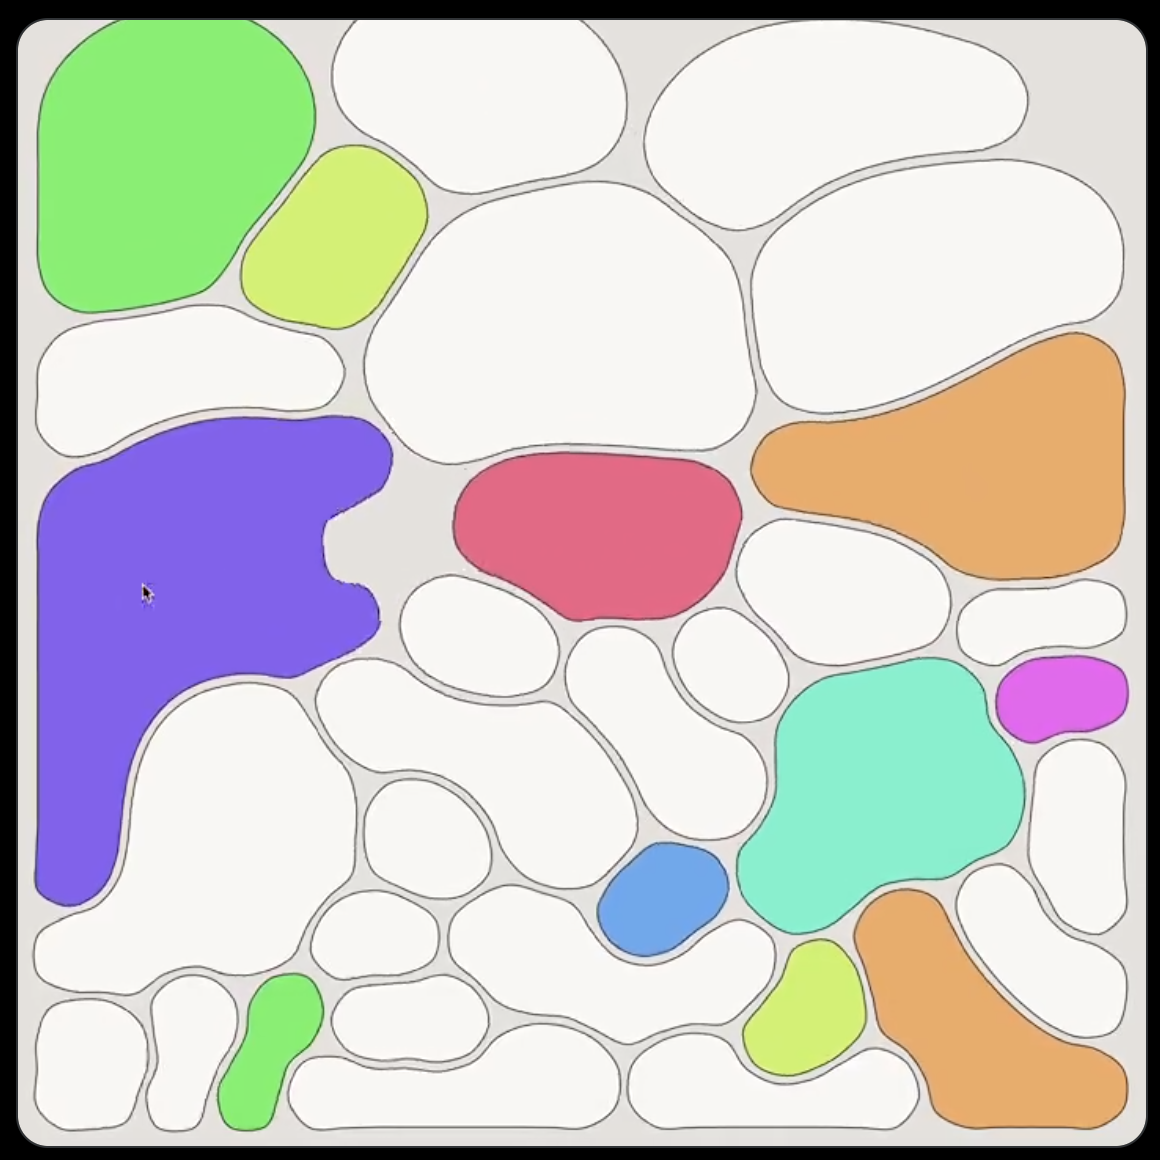
\includegraphics[width=0.4\textwidth]{figures/juhani.png}
  \caption{Juhani Halkomäki work with soft-body physics.}
  \label{fig:juhani}
  \Description{A screenshot with colorful blobs pressed together inside a container}
\end{figure}

\section{Background}

This project touches on many different research topics. Because of this, this section is divided into subsections to keep things organized.

\subsection{Minimalism vs embellishments in visualization design} \label{background-minimalism}

In his seminal work, \textit{The Visual Display of Quantitative Information}, Edward Tufte laid some of the principles that promote minimalism in chart design. To propose his "Theory of Data Graphics", Tufte establishes first the core concept of \textit{data-ink ratio}, which is central to his principles of graphical minimalism \cite{tufte2001visual}:

\begin{displaymath} 
    \text{Data-ink ratio} = \frac{\text{data-ink}}{\text{total ink used to print the graphic}}
\end{displaymath}

Based on this \textit{data-ink ratio} concept, his principles are laid down as follows:

\begin{itemize}
    \item Above all else show the data.
    \item Maximize the data-ink ratio.
    \item Erase non-data-ink.
    \item Erase redundant data-ink
    \item Revise and edit
\end{itemize}

Tufte strongly opposes the use of "decoration" in chart design, which originates, according to him, in the belief, held by many graphic artists, that statistics are "boring", and thus would need to be enlivened and animated by the use of embellishments \cite{tufte2001visual, tufte1990envisioning}. Tufte often labels these embelishments or decorations as "chartjunk" \cite{tufte2001visual}, using the work of Nigel Holmes as a counter-example of good chart design.

Unsurprisingly, Nigel Holmes proposes a very different approach to chart design.

Somewhat opposite to this view of chart design lies the work of Nigel Holmes. Holmes calls Tufte views as... concept of joyful infographics.

Memorability studies.

Emotional value. Dorsey. Impressionism.

Tufte's principles
* Lie factor
* the number of information-carrying (variable) dimensions depicted should not exceed the number of dimensions in the data.
exemplo do Playfair

know the rules to know when to break them?


\subsection{Soft-Body Physics} \label{background-soft-body}

Physics game engine in general

Integrators

In the end it's Particle Systems. The seminal work is \cite{particle-ReevesW.T.1983PSTf}.

Terzopoulos, seminal work.

Physically based deformable models have two decades of history
in Computer Graphics: since Lasseter’s discussion of
squash and stretch [1] and, concurrently, Terzopoulos et. al’s
seminal paper on elastically deformable models [2], numerous
researchers have partaken in the quest for the visually
and physically plausible animation of deformable objects and
fluids. This inherently interdisciplinary field elegantly combinesNewtonian
dynamics, continuum mechanics, numerical
computation, differential geometry, vector calculus, approximation
theory and computer graphics (to name a few) into
a vast and powerful tool kit, which is being further explored
and extended.\cite{NealenAndrew2006PBDM}


\subsection{Soft-Body in Visualization}



\subsection{Uncertainty in Visualization}

in policy analysis, economics. Morgenstern.

There has been many studies / techniques aimed at visualizing uncertainty. \cite{Padilla-uncertainty-chapter}, \cite{HullmanJessica2019IPoE}




The uncertainty we are trying to convey here is not a measured statistical uncertainty, but rather a more fundamental, epistemic one. This uncertainty derives from bla bla Ben Jones. \cite{ben-jones-data-pitfalls}.


\subsection{Visualization Evaluation} \label{section:vis-eval}

One central process in the visualization pipeline model is the mapping of data variables to visual variables \cite{readings-infovis-shneiderman}. Researchers in Information Visualization have long investigated the effectiveness of these visual mappings in terms of graphical perception \cite{HeerJeffrey2010Cgpu-bostock-amazon-turk}. Their study contributed to the development of many rankings of visual variables (citar Tamara, Ware?)

The seminal work in this area is Cleveland and McGill's study of graphical perception using a set of perceptual tasks, where subjects were asked to estimate the proportionality between pairs of visual marks across different types of spatial encodings (angle, length, position)  \cite{ClevelandWilliamS.1984GPTE}.

Kosara and Correll propose important criticism of the state of information visualization research.

Proposed a framework of tasks.

Bremer and Munzner developed a multi-level typology of abstract visualization tasks, trying to bridge the gap between low-level and high-level classification systems \cite{BrehmerMatthew2013AMTo}.

Compared perception for five different charts.

More criticism, from McColeman et al. \cite{McColemanCaitlynM.2022RtRo-rethinking-visual-channels}
An existing ranking of these
visual channels is based on how accurately participants could report the ratio between two depicted values. There is an assumption
that this ranking should hold for different tasks and for different numbers of marks. However, there is surprisingly little existing work that
tests this assumption, especially given that visually computing ratios is relatively unimportant in real-world visualizations, compared
to seeing, remembering, and comparing trends and motifs, across displays that almost universally depict more than two values.

Quadri and Rosen surveyed hundreds of perception-focused visualization studies, creating a practical taxonomy of studies based on Amar et al. low-level task taxonomy.

Criticism, such as Kosara \cite{kosara2016empire}, Michael Correll \cite{CorrellProgressVis}.

Isenberg et al. reflect that, although there have been improvements, the \textit{general level of rigor of reporting evaluations is still too low} \cite{IsenbergTobias2013ASRo}.

Regarding crowdsourced experiments, Bostock ...\cite{HeerJeffrey2010Cgpu-bostock-amazon-turk}.

One common problem in evaluation studies is ecological validity. with the use of crowdsourcing, by relying on the participants' standard displays, Heer and Bostock suggest that experimental control could effectively be swapped for ecological validity \cite{HeerJeffrey2010Cgpu-bostock-amazon-turk}.

Heer and Bostock's seminal work demonstrated the viability of crowdsourcing for testing graphical perception, citing the increase in the numbers and diversity of the subjects as one of its advantages.
We replicate prior laboratory studies on spatial data encodings
and luminance contrast using crowdsourcing techniques.
Our new results match previous work, are consistent
with theoretical predictions [21], and suggest that
crowdsourcing is viable for testing graphical perception

There is something wrong with
every methodological technique, which can often be compensated
by combining techniques. \cite{HeerJeffrey2010Cgpu-bostock-amazon-turk}

It is interesting to note that, although user experience and user performance are among the most common studies in the field of human-computer interaction, Isenberg et al. express their surprise on the low number of scenarios and papers that fell in this category in their survey \cite{IsenbergTobias2013ASRo}.

O'Brien et al. propose a refined version UES bla bla \cite{O’BrienHeatherL.2018Apat-engagement}.



\subsection{Vis in Government}


Government:

However, just as with the “digital divide”, these divisions don’t simply stop or be resolved with the provision of digital (or data) “access”. What is necessary as well is that those for whom access is being provided are in a position to actually make use of the now available access (to the Internet or to data) in ways that are meaningful and beneficial for them. \cite{Gurstein_2011-open-data-use}


\subsection{Emotional Value}

By rendering a real-time simulation, animation becomes a natural part of the visualization, and animations can engage emotions, sparking greater interest or enjoyment \cite{HeerJ.2007ATiS-animation}.

\section{Method}

\subsection{Building a Soft-body Simulation}

In this project, we propose an information visualization technique in which data points are visually represented as dynamical deformable bodies in a physically realistic simulation (with a focus on visually plausibility, rather than scientific accuracy).

As mentioned in \ref{background-soft-body}, there are many approaches to implementing a simulation of soft-bodies \cite{NealenAndrew2006PBDM, book-deformable-objects}. We employ a mixed approach, representing the deformable objects -- we will can them \textit{blobs} -- as particle systems of a set of point-masses connected by massless springs and also subjected to a pressure force, responsible for maintaining the original circular shape.

The study of physically-based deformable models is a fascinating interdisciplinary field that combines "Newtonian dynamics, continuum mechanics, numerical computation, differential geometry, vector calculus, approximation theory and computer graphics (to name a few)" \cite{NealenAndrew2006PBDM}. Given this and considering the pedagogical nature of a master's degree project, we took the opportunity to dive into and understand how physical simulations for computer graphics work. Thus, we decided not to use a readily available soft-body simulation in a framework such as Unity, or any of the physics libraries available to the Web platform, but to develop our own real-time simulation and simplified physics engine from the ground up in Javascript, starting from our own vector library.

The Web platform was chosen because of its ubiquity, graphics and interaction capabilities, and easy, immediate distribution of content.

Therefore, a CPU 2D soft body physics real-time simulation was developed for Web Browsers using Javascript. The HTML Canvas 2D Context\footnote{https://www.w3.org/2015/04/2dcontext-lc-sample.html} is used for rendering, and the animation is achieved with the `requestAnimationFrame` API\footnote{https://html.spec.whatwg.org/multipage/imagebitmap-and-animations.html\#dom-animationframeprovider-requestanimationframe}, both part of W3C Web Standards.

In this section, we provide the details of our implementation\footnote{Source code is available at https://github.com/tiago-kth/master-thesis.}.

\subsubsection{Data Structures}

The very first structure needed for our simulation is a Vector library. This library, implemented as a JavaScript class \texttt{Vec}, provides the data structures necessary to represent vectors (and points), storing the vectors' \texttt{x} and \texttt{y} attributes, and also provides a variety of vector operations, such as addition, subtraction, scalar product, projection, calculating the vector's magnitude, obtaining a unit vector in the vector's direction etc. Also, to make it easy to debug and understand the behavior of the system, a method to visualize the vector was also developed. To illustrate how the library works, consider the following operations that define two vectors, adds them together and displays all three vectors anchored at the center of the canvas:

\begin{verbatim}

let p0 = new Vec(W/2, H/2);

let vec_a = new Vec(300, 300);
let vec_b = new Vec(100, -200);
let vec_c = Vec.add(vec_a, vec_b);

// ctx holds the reference to the rendering context

vec_a.display(ctx, p0, "blue");
vec_b.display(ctx, p0, "green");
vec_c.display(ctx, p0, "red");

\end{verbatim}

The resulting rendered image is show in figure \ref{fig:vectors}.

\begin{figure}[h]
  \centering
  \includegraphics[width=0.45\textwidth]{figures/vector-library.png}
  \caption{A basic vector addition with the \texttt{Vec} library.}
  \label{fig:vectors}
  \Description{Three vectors on a grid, one vector labeled as vec_a, another as vec_b and a third (the sum of vec_a and vec_b) as vec_c}
\end{figure}

With the vector library in place, we move to the main data structures of our simulation. The physics engine we developed for this project was the "mass-aggregate" engine type -- an engine that treats objects as collections of simple point-masses \cite{game-physics-millington}. In this way, our deformable objects, or blobs, represent collections of point-masses, or particles. A \texttt{Particle} class therefore was implemented with several attributes that are usually present in any Particle System and that are relevant to the simulation (\textit{position}, \textit{velocity}, \textit{acceleration} etc.) and to the particles' rendering (\textit{size}, \textit{color}, \textit{transparency} etc.) \cite{particle-ReevesW.T.1983PSTf}.

The particles are, naturally, essential to the simulation, because they are the objects that effectively change position, velocity and acceleration. The forces are applied to them, and collisions happen to them. Therefore, they are the most complex data structure in this simulation. A summary of their main properties is listed on table \ref{tab:particle}.

\begin{table}
  \caption{Particles' attributes}
  \label{tab:particle}
  \begin{tabularx}{\textwidth}{rX}
    \toprule
    \texttt{position} & vector that holds the particle's current \texttt{x} and \texttt{y} position\\
    \texttt{velocity} & vector that holds the particle's current velocity\\
    \texttt{acceleration} & vector that holds the particle's current acceleration\\
    \texttt{force\_acum} & vector that accumulates the sum of all forces applied to the particle at a given frame\\
    \texttt{blob} & reference to the blob object that contains the particle\\
    \texttt{springs} & references to the outer springs connected to the particle\\
    \texttt{collider\_center} & vector that holds the position of the particle's corresponding external collider (used to evaluate collisions on the blob's external surface)\\
    \texttt{internal\_collider\_center} & vector that holds the position of the particle's corresponding internal collider (used to evaluate collisions on the blob's internal surface)\\
    \texttt{immediate\_neighbors} & references to the particle's immediate neighbors in the same blob (used in the collision system)\\
    \texttt{grid\_cell} & id of the grid cell that currently contains the particle (used to improve the performance of the collision system)\\
    \bottomrule
    \end{tabularx}
\end{table}

The particles are connected together by springs. The springs are responsible for keeping the blob together, by applying equal and opposite forces to each of its connected particles, as we will discuss in section \ref{section:forces}. They are also implemented as a specific class, \texttt{Spring}, and a summary of their main properties is listed on table \ref{tab:spring}.

\begin{table}
  \caption{Springs' attributes}
  \label{tab:spring}
  \begin{tabularx}{\textwidth}{rX}
    \toprule
    \texttt{p1} & a reference to one of the particles to which the spring is connected\\
    \texttt{p2} & a reference to the other particle to which the spring is connected\\
    \texttt{rest\_length} & a value that represents the original length of the spring, when no force is applied to it\\
    \texttt{current\_length} & a value that represents the current length of the spring, obtained by calculating the distance between \texttt{p1} and \texttt{p2}.\\
    \texttt{normal} & unit vector perpendicular to the spring, that is used to apply the pressure force\\
    \bottomrule
    \end{tabularx}
\end{table}

Finally, the deformable bodies, the blobs, have their own data structure as well: the \texttt{Blob} class. Since the blobs represent the actual data points in a similar way as bubbles in a Bubble Chart, their size is defined by its corresponding data value, according to a scale function. According to their size, the number and initial positions of particles is defined, which in turn define the number and initial length of the springs. We will detail this process shortly, in section \ref{section:initial-setup}, but first we list the main properties of the \texttt{Blob} class on table \ref{tab:blob}.

\begin{table}
  \caption{Blobs' attributes}
  \label{tab:blob}
  \begin{tabularx}{\textwidth}{rX}
    \toprule
    \texttt{R} & the initial and ideal blob radius, when no force is applied to its particles.\\
    \texttt{rest\_area} & the initial and ideal blob area, which corresponds to the area of a circle with radius \texttt{R}.\\
    \texttt{current\_area} & value that keeps track of the current blob's area, evaluated with the Shoelace Formula.\\
    \texttt{center} & vector that keeps track of the current position of the blob's center\\
    \texttt{particles} & references to the particles that make up the blob.\\
    \texttt{springs} & references to the springs that make up the blob.\\
    \bottomrule
    \end{tabularx}
\end{table}

\subsubsection{Initial Setup}\label{section:initial-setup}

Similarly to how one would proceed with a Bubble Chart, we are representing data points to area objects, encoding some numerical data variable to the objects' areas. Our first step is to find a suitable scaling function to map those data values to actual areas. Since the space on the canvas is limited, it is interesting to represent the sum of all values as a percent of the available canvas area. Having the total value mapped to an area, we can use a simple rule of three to obtain the individual target areas. Depending on the nature of the dataset, one can also use more meaningful maps, that might convey extra information to the reader. For example, in our dataset of government expenditures as percentages of the GDP, we can map the percentage values to areas that correspond to the same percentage of the total available screen area. In this way, the container's area would represent the country's GDP, and the blobs' areas would be a direct visual representation of the actual expenditure in terms of percentages of the GDP.

Since the blobs will initially assume a circular shape, once we have the target areas of each blob, we can determine their radii using the circle's area formula. We then populate the blob's perimeter with adjacent particles, calculating the number of necessary particles based on the blob's radius and the particles' radius (a parameter of the simulation). Next, we connect all adjacent particles and every other particle with springs. The algorithm \ref{algo:init} details this process. Figure \ref{fig:one-blob} shows what an initialized blob looks like, with particles rendered as circles, and springs rendered as straight lines. In our prototype's debug mode, it is possible to render the particles and springs as shown in the figure, or the whole blob as a polygon made of lines connecting the centers of the particles.

\begin{algorithm}
\caption{Blob Initialization} \label{algo:init}
\begin{algorithmic}[1]
\State $\theta \gets \arctan\left(\frac{2 * \text{PARTICLE\_RADIUS}}{blob\_radius}\right)$
\State $n \gets \left\lfloor \frac{2 * \pi}{\theta} + 0.5 \right\rfloor$ \Comment{Rounds to the nearest integer, to have a valid number of particles}
\State $\theta \gets \frac{2 * \pi}{n}$ \Comment{Recalculates the angle between particles considering the new number of particles}

\Function{vectorFromAngle}{$magnitude, angle, p_0$}
    \State $x \gets p_0.x + \cos(angle) * magnitude$
    \State $y \gets p_0.y - \sin(angle) * magnitude$
    \State \Return $\text{new Vector}(x, y)$
\EndFunction

\For {$i \gets 0$ to $n-1$}
    \State $position \gets vectorFromAngle(blob\_radius, \theta * i, blob\_center)$
    \State $p \gets \text{new Particle}(position)$
    \State $\text{add } p \text{ to } particles$ \Comment{the blob's particles list/array}
\EndFor

\For {$i \gets 0$ to $n-1$}
    \State $next\_index \gets \begin{cases}
    0 & \text{if } i = particles.length - 1 \\
    i + 1 & \text{otherwise}
    \end{cases}$
    
    \State $s \gets \text{new Spring}(particles[i], particles[next\_index])$\Comment{a spring connecting neighboring particles}
    \State $\text{add } s \text{ to } particles[i].springs$ \Comment{the particle's list/array of springs connected to it}
    \State $\text{add } s \text{ to } particles[next\_index].springs$  
    \State $\text{add } s \text{ to } springs$ \Comment{the blob's springs list/array}
    
    \State $s2 \gets \text{new Spring}(particles[i], particles[(i + 2) \mod particles.length])$\Comment{a spring connecting every other particle}
    \State $\text{add } s2 \text{ to } springs$ \Comment{the blob's springs list/array}
\EndFor

\end{algorithmic}
\end{algorithm}

\begin{figure}[h]
  \centering
  \includegraphics[width=0.33\textwidth]{figures/one-blob.png}
  \caption{A blob's structure: its particles (circles) and springs (lines).}
  \label{fig:one-blob}
  \Description{A big circle made of adjacent smaller circles and lines connecting their centers}
\end{figure}

\subsubsection{Simulation overview}

The main animation loop is comprised of the following steps:

\begin{enumerate}
    \item Compute and accumulate forces
    \item Integrate
    \item Handle Collisions
    \item Satisfy Boundary Constraints
    \item Render
\end{enumerate}

We address each of these steps in the following sections.

\subsubsection{Forces}\label{section:forces}

We compute and accumulate three forces, successively: the spring force, the pressure force and the gravity force.

\paragraph{Spring Force}

As in any mass-spring system, springs exert equal and opposite forces on each object attached to them. According to Hooke’s law, the force exerted by the spring is determined by its displacement (stretching or compression) from its rest length and the spring constant \cite{physics-game-developers-oreilly}:

\[F_s = -k_s \Delta l\]

In this way, the spring constant quantifies the relationship between the force exerted by the spring and its displacement ($\Delta l = l - l_rest$). Hooke’s law indicates that the displacement is directly proportional to the applied force. The negative sign means that the force acts in the opposite direction of the displacement. 

In our simulation, all springs have the same spring constant, which is one of the simulation's key parameters, as we shall see later. As we can see in Table \ref{tab:spring}, the \texttt{Spring} object stores the original spring's length, that is, its \textit{rest length}, $l_{rest}$, as well as references to the particles connected to it. These \texttt{Particle} objects, in turn, keep track of their current position, which we will call $\vec{p_1}$ and $\vec{p_2}$. Hooke's law then becomes (acting on particle 1):

\[\vec{F_{s1}} = -k_s (|\vec{p_1} - \vec{p_2}| - l_{rest}) \hat{l} \]

Where 

\[\hat{l} = \frac{\vec{p_1} - \vec{p_2}}{|\vec{p_1} - \vec{p_2}|} \]

Similarly, on particle 2 we have an opposite force of:

\[\vec{F_{s2}} = k_s (|\vec{p_1} - \vec{p_2}| - l_{rest}) \hat{l} \]

A real spring will not oscillate forever -- that is, beyond forces, a real spring also experiences drag \cite{game-physics-millington}. To simulate drag in a numerical simulation we add a damping component, proportional to the the relative velocity of the connected particles, $\vec{v_1}$ and $\vec{v_2}$, multiplied by a damping parameter $k_d$, another important simulation parameter.

\[\vec{F_{d1}} = -k_d (\vec{v_1} - \vec{v_2}) \cdot \hat{l} ) \hat{l} \]
\[\vec{F_{d2}} =  k_d (\vec{v_1} - \vec{v_2}) \cdot \hat{l} ) \hat{l} \]

Computationally, our procedure is described in Algorithm \ref{algo:spring-force}.

\begin{algorithm}
\caption{Spring force computation} \label{algo:spring-force}
\begin{algorithmic}[1]

\For {every $blob$ of all $blobs$}

    \State $springs \gets \text{list/array of all springs in } blob$

    \For {every $spring$ of $springs$}
        \State $k_s \gets \text{STIFFNESS parameter}$
        \State $k_d \gets \text{DAMPING parameter}$
        \State $\vec{p_1} \gets \text{position of particle 1 of }spring$
        \State $\vec{p_2} \gets \text{position of particle 2 of }spring$
        \State $\vec{L} \gets \vec{p_1} - \vec{p_2}$
        \State $l \gets |\vec{L}|$ \Comment{Current length}
        \State $\hat{l} \gets \frac{\vec{L}}{l}$
        \State $l_{rest} \gets \text{rest length of }spring$

        \State $\vec{v_1} \gets \text{velocity of particle 1 of }spring$
        \State $\vec{v_2} \gets \text{velocity of particle 2 of }spring$
        \State $\vec{v_{1,2}} \gets \vec{v_1} - \vec{v_2}$

        \State $f \gets (l - l_{rest}) k_s + (\vec{v_{1,2}} \cdot \hat{l}) k_d $

        \State $\vec{F} \gets f \hat{l}$

        \State \text{add $-\vec{F}$ to $force\_accumulator$ of particle 1}
        \State \text{add $\vec{F}$ to $force\_accumulator$ of particle 2}
        \State \text{store $l$ in $spring.current\_length$} \Comment{This will be used to compute the Pressure Force}
        
    \EndFor
\EndFor
\end{algorithmic}
\end{algorithm}

Figure \ref{fig:spring-force} illustrates the spring forces acting on the blob's particles.

\begin{figure}[h]
  \centering
  \includegraphics[width=0.33\textwidth]{figures/spring-force.png}
  \caption{Spring forces}
  \label{fig:spring-force}
  \Description{A big circle made of adjacent smaller circles and lines connecting their centers, with vectors representing the spring forces on the smaller circles}
\end{figure}

\paragraph{Pressure Force}

We included a pressure component in our model to perform the critical role of helping to keep the overall blob's shape and to avoid the blob's collapse or having its borders flipping over one another.

\begin{figure}[h]
  \centering
  \includegraphics[width=0.33\textwidth]{figures/flipped-over-blob.png}
  \caption{A blob with crossed edges (highlighted in red)}
  \label{fig:flipped-over}
  \Description{A big circle made of adjacent smaller circles and lines connecting their centers. It has a couple of edges crossed over.}
\end{figure}

To model this force, we consider that the blob is filled with an ideal gas, following Matyka \& Ollila implementation \cite{pressure-MaciejMatyka2004PMoS, matyka2004implement}. The empirical form of the ideal gas law is well-known:

\[PV = nRT \]

Where $P$ is the pressure, $V$ is the volume, $n$ is the amount of substance, $R$ is the ideal gas constant and $T$ is the temperature. In our simplified model, the temperature is constant. Hence, the $nRT$ term can be considered constant, which we will call $k_p$, the pressure constant, one important simulation parameter. Furthermore, we are dealing with a 2D model, and thus the volume can be represented by the blob's area, $A_b$:

\begin{equation} \label{eq:pressure}
P = A_b^{-1} k_g
\end{equation}


In our simulation, we are interested in the normal force $F_p$ related to the pressure:

\[P = \frac{F_p}{A} \]

In our 2D model, the pressure translates to a force applied not to an area, but to a line segment represented by the blob's springs, that has a length of $l$. The force is applied in a normal direction, given by the unit vector $\hat{n}$:

\[\vec{F_p} = Pl\hat{n} \]

Applying equation \ref{eq:pressure} yields:

\begin{equation} \label{eq:pressure-complete}
\vec{F_p} = \frac{l}{A_b} k_g \hat{n}
\end{equation}

Where $\hat{n}$ is a normal unit vector to the spring. Considering the positions of the spring's particles $p_1$ and $p_2$, and the length $l$ of the spring, we have the unit vector $\hat{l}$ in the spring's direction:

\[
p_1 = \begin{bmatrix} x_1 \\ y_1 \end{bmatrix}, \quad
p_2 = \begin{bmatrix} x_2 \\ y_2 \end{bmatrix}, \quad
\text{ and then } \hat{l} = \begin{bmatrix} (x_2-x_1)/l \\ (y_2-y_1)/l \end{bmatrix}
\]

In this way, the normal unit vector becomes:

\[
\hat{n} = \begin{bmatrix} -(y_2-y_1)/l \\ (x_2-x_1)/l \end{bmatrix}
\]

From equation \ref{eq:pressure-complete}, we can notice that when the blob is compressed, its area becomes smaller, producing a stronger pressure force that will try to restore the blob's original shape.

Our computational procedure is described in Algorithm \ref{algo:pressure-force}.

\begin{algorithm}
\caption{Pressure force computation} \label{algo:pressure-force}
\begin{algorithmic}[1]

\Function{getNormal}{$spring$}
    \State $l \gets spring.current\_length$
    \State $\vec{p_1} \gets \text{position of particle 1 of }spring$
    \State $\vec{p_2} \gets \text{position of particle 2 of }spring$
    \State $x_1 \gets p_1.x$
    \State $y_1 \gets p_1.y$
    \State $x_2 \gets p_2.x$
    \State $y_2 \gets p_2.y$
    \State $n.x \gets -(y_2-y_1)/l$
    \State $n.y \gets (x_2-x_1)/l$
    \State \Return $\hat{n}$
\EndFunction

\For {every $blob$ of all $blobs$}

    \State $k_p \gets \text{PRESSURE parameter}$
    \State $A_b \gets blob \text{ current area}$
    
    \State $springs \gets \text{list/array of all springs in } blob$

    \For {every $spring$ of $springs$}

        \State $l \gets spring.current\_length$

        \State $f_p \gets \frac{l}{A_b}k_p $

        \State $\hat{n} \gets getNormal(spring)$

        \State $\vec{F_p} \gets f_p \hat{n}$

        \State \text{add $\vec{F_p}$ to $force\_accumulator$ of particle 1 of $spring$}
        \State \text{add $\vec{F_p}$ to $force\_accumulator$ of particle 2 of $spring$}
        
    \EndFor
\EndFor
\end{algorithmic}
\end{algorithm}

Figure \ref{fig:pressure-force} illustrates two examples of pressure forces acting on the blobs particles.

\begin{figure}[h]
  \centering
  \includegraphics[width=0.4\textwidth]{figures/pressure-force.png}
  \includegraphics[width=0.4\textwidth]{figures/pressure-force-2.png}
  \caption{Pressure force}
  \label{fig:pressure-force}
  \Description{Two pictures of big circles made of adjacent smaller circles and lines connecting their centers. Pink outwards vectors indicate the pressure force.}
\end{figure}

\paragraph{Gravity Force}

A gravity force is added to the simulation as well. Its computation is far simpler than the other two forces since the force is the same for every particle of the simulation. It is a direct application of Newton's Second Law:

\[ \vec{F} = m\vec{a}\]

In our simulation, we can consider the acceleration $\vec{a}$ as a downward pointing vector with magnitude equal to a gravity constant, $G$ which is another simulation parameter:

\[
\vec{a} = \vec{g} = \begin{bmatrix} 0 \\ G \end{bmatrix}
\]

Computationally, we can simply loop over all particles and add the same force to each particle's force accumulator (algorithm \ref{algo:gravity-force}). Figure \ref{fig:gravity-force} shows this force acting on the blob's particles.

\begin{algorithm}
\caption{Gravity force computation} \label{algo:gravity-force}
\begin{algorithmic}[1]

\For {every $blob$ of all $blobs$}
    
    \State $particles \gets \text{list/array of all particles in } blob$

    \For {every $particle$ of $particles$}

        \State $m \gets \text{property $mass$ of} particle$

        \State $G \gets \text{GRAVITY parameter}$

        \State $\vec{g} \gets [0, G]$

        \State $\vec{F_g} \gets m\vec{g}$

        \State \text{add $\vec{F_g}$ to $force\_accumulator$ of $particle$}
        
    \EndFor
\EndFor
\end{algorithmic}
\end{algorithm}

\begin{figure}[h]
  \centering
  \includegraphics[width=0.4\textwidth]{figures/gravity-force.png}
  \caption{Gravity force}
  \label{fig:gravity-force}
  \Description{A picture of a big circle made of adjacent smaller circles and lines connecting their centers. Green vectors pointing downwards indicate the gravity force.}
\end{figure}

\subsubsection{Integrator}

A key component of every numerical simulation is the numerical integrator. In a real-time simulation, the motion of objects is not controlled by pre-defined motion sequences. Instead, the simulation depends on a physics model, equations of motion, and a differential equation solver to determine the objects' movements as the simulation unfolds \cite{physics-game-developers-oreilly}.

Therefore, our integrator is responsible for updating each particle's position $p$, velocity $v$, and acceleration $a$ in each frame. We know that the particle's velocity is defined as the change of its velocity over a time period. If we could make this time period infinitely small, we could calculate the exact velocity at any point in time \cite{game-physics-millington}:

\[
    v = \lim_{\Delta t\to 0} \frac{\Delta p}{\Delta t} = \frac{dp}{dt} = \dot{p}
\]

Since acceleration represents the rate of change in velocity, we can express it in a similar way \cite{game-physics-millington}:

\begin{equation}
\label{eq:acceleration-derivative}
     a = \lim_{\Delta t\to 0} \frac{\Delta v}{\Delta t} = \frac{dv}{dt} = \frac{d^2v}{dt^2} = \ddot{p}   
\end{equation}

If we know the particle's acceleration ($\ddot{p}$) and its current velocity ($\dot{p})$, we can work out its next velocity $\dot{p}'$ at some given point by integrating the acceleration expression in equation \ref{eq:acceleration-derivative}:

\begin{equation}
\label{eq:integrator-velocity}
    \dot{p}' = \dot{p} + \ddot{p}t
\end{equation}

And then we can find the particle's next position $p'$ by computing the second integral of the acceleration:

\begin{equation}
\label{eq:integrator-position}
    p'= p + \dot{p}t = + \ddot{p} \frac{t^2}{2}
\end{equation}

In this way, at each frame, after computing all forces acting on each particle, we will determine the particle's acceleration using Newton's second law of motion, $\vec{a} = \vec{F}m^{-1}$. We then use equations \ref{eq:integrator-velocity} and \ref{eq:integrator-position} to update the particle's position and velocity. We can notice that these equations need a time interval, and in our prototype we use a value defined by a simulation parameter, so we can control the speed of the simulation and quickly adjust the simulation when instabilities arise.

To improve stability, we use a slightly different integration method. Based on the Verlet integration method \cite{VerletLoup1967C"oC}, which is used extensively in molecular dynamics simulations \cite{jakobsen2001advanced}, the so-called Velocity Verlet method combines simplicity with good numerical precision \cite{SwopeWilliamC.1982Acsm-velocity-verlet, wiki:Verlet_integration}. The algorithm \ref{algo:integrator} illustrate our integration procedure based on this method.

\begin{algorithm}
\caption{Integrator} \label{algo:integrator}
\begin{algorithmic}[1]

\For {every $blob$ of all $blobs$}
    
    \State $particles \gets \text{list/array of all particles in } blob$

    \For {every $particle$ of $particles$}

        \State $\vec{p} \gets \text{property $position$ of } particle$
        \State $\vec{v} \gets \text{property $velocity$ of } particle$
        \State $\vec{a} \gets \text{property $acceleration$ of } particle$
        \State $\vec{F} \gets \text{property $force\_accumulator$ of } particle$
        \State $t \gets \text{TIME-STEP parameter}$ 
        \State $d_v \gets \text{VELOCITY DAMPING parameter}$ 

        \State $\vec{p'} \gets \vec{p} + \vec{v}t + 0.5t^2\vec{a}$
        \State $\vec{a'} \gets \vec{F} m^{-1}$
        \State $\vec{v'} \gets d_v\vec{v} + (\vec{a} + \vec{a'})/2$

        \State $\vec{p} \gets \vec{p'}$
        \State $\vec{v} \gets \vec{v'}$
        \State $\vec{a} \gets \vec{a'}$

        \text{clear $force\_accumulator$ of $particle$}
    \EndFor
\EndFor
\end{algorithmic}
\end{algorithm}

Notice that when the velocity is updated, the current velocity is multiplied by a damping factor $d_v$, which is a simulation parameter. It controls how much velocity is left after the update. Thus, this damping factor has the role of removing energy added through numerical instability in the integrator, and can also be used to simulate real-world drag \cite{game-physics-millington, physics-game-developers-oreilly}.

\subsubsection{Collision detection}

One important aspect of our prototype is the interaction between the blobs. We expect the blobs to push and shove each other, and that, in practice, translates into detecting and resolving collisions between particles.

The particles are represented as circles centered on their \texttt{position} property with radius \texttt{r}. To detect collisions, the collision system must first compute the interpenetration between pairs of particles. The penetration can be calculated as the difference between the distance from one particle to the other and the minimum distance before the particles start overlapping (the sum of their radii):

\[
\vec{d} = \vec{p_1} - \vec{p_2}
\]

\[
d_{MIN} = r_1 + r_2 = 2r
\]

Figure \ref{fig:collision-detection} illustrates the three possible situations regarding interpenetration.

\begin{figure}[h]
  \centering
  \includegraphics[width=\textwidth]{figures/scheme-collision.png}
  \caption{Collision detection}
  \label{fig:collision-detection}
  \Description{A scheme showing the three possible situations regarding the position of a pair of circles.}
\end{figure}

It would be unnecessarily expensive to check every possible combination of pairs of particles at each frame. Instead, we use a grid system of cells to check possible collisions only between a given particle and the particles in its cell (or in the eight surrounding cells). Figure \ref{fig:collision-grid} illustrates this idea, showing the particles of two different blobs, and highlighting the particles (in pink) that are in the same cell or in the immediate surrounding cells of a given particle (in blue).

\begin{figure}[h]
  \centering
  \includegraphics[width=0.5\textwidth]{figures/collision-grid.png}
  \caption{Grid system for collision detection}
  \label{fig:collision-grid}
  \Description{Two blobs made up of particles where one particle is highlighted in blue, and all particles within its cell and the surrounding cells are highlighted in pink.}
\end{figure}

Given the small radius of the particles, it may happen that, from one frame to another, one particle could completely traverse another particle. In this situation, the distance between the two particles would remain above the minimum distance ($2r$) in both frames, and the collision system would not flag a collision. But this could cause part of one blob to cross the boundaries of another, which is very undesirable. To solve this situation, we use larger circles as colliders. Each particle has a corresponding collider, placed in such a way that their outer borders coincide (Figure \ref{fig:collision-detection-colliders}).

\begin{figure}[h]
  \centering
  \includegraphics[width=0.5\textwidth]{figures/collision-detection-colliders.png}
  \caption{Actual colliders used in the collision detection system}
  \label{fig:collision-detection-colliders}
  \Description{Two blobs made up of particles where some of the particle's colliders (larger circles) are represented.}
\end{figure}

Therefore, the first step of the collision system is to loop over all particles and compute distances to other particles (to be more precise, to compute the distance between their colliders) in its vicinity (algorithm \ref{algo:collision-detection}. If the distance is less or equal to the sum of the colliders' radii, that is if $penetration = d_{MIN} - d \ge 0$, a collision is registered, along with the collision's contact normal $\hat{d}$ (a unit vector in the direction that connects the centers of the colliders).

\begin{algorithm}
\caption{Collision detection} \label{algo:collision-detection}
\begin{algorithmic}[1]

\For {every $particle_1$ of all $particles$}

    \State text{Get current cell index, and the indices of the neighboring cells}
    \State $neighboring\_particles \gets \text{list/array of particles in neighboring cells}$

    \For {every $particle_2$ of $neighboring\_particles$}

        \State $\vec{c_1} \gets \text{center of collider of } particle_1$
        \State $\vec{c_2} \gets \text{center of collider of } particle_2$
        \State $r_1 \gets \text{radius of collider of } particle_1$
        \State $r_2 \gets \text{radius of collider of } particle_2$
        \State $\vec{d} \gets \vec{c_1} - \vec{c_2}$
        \State $d \gets |\vec{d}|$
        \State $\hat{d} \gets \frac{\vec{d}}{|\vec{d}|}$
        \State $d_{MIN} = r_1 + r_2$
        \State $penetration \gets d_{MIN} - d$
        \If{$penetration \ge 0$}
            \State \text{register collision of $particle_1$ and $particle_2$ with contact normal $\hat{d}$}
            \State \text{add collision to collisions registry}
        \EndIf
    \EndFor
\EndFor
\end{algorithmic}
\end{algorithm}

Once all collisions are detected in a given frame, it is necessary to resolve the collisions and the penetrations. 

\paragraph{Resolving interpenetrations}

A penetration is resolved by simple projection \cite{jakobsen2001advanced, game-physics-millington}. The particles that are interpenetrating must be moved along the direction of their contact normal (evaluated when the collision was detected). If $\Delta p_1$ and $\Delta p_2$ are the scalar distances that each particle must move to eliminate the interpenetration, then:

\[
\Delta p_1 + \Delta p_2 = penetration
\]

Normally the relationship between the two distances would be given by the ratio of their masses \cite{game-physics-millington}:

\[
m_1\Delta p_1 = m_2\Delta p_2
\]

Combining these equations, we have:

\[
\Delta p_1 = \frac{m_2}{m_1 + m_2} penetration
\]

and

\[
\Delta p_2 = \frac{m_1}{m_1 + m_2} penetration
\]

But in our simulation, all particles have the same mass, thus:

\[
\Delta p_1 = \Delta p_2 = \frac{penetration}{2}
\]

In terms of the vector change in the position of the particles, the expressions become:

\[
\Delta \vec{p_1} = \frac{penetration}{2} \hat{n}
\]

and

\[
\Delta \vec{p_2} = -\frac{penetration}{2} \hat{n}
\]

\paragraph{Resolving collisions}

We resolve collisions by relying on classical, Newtonian impact principles. First, we compute, for each collision, the \textit{separating velocity}, that is, the total speed at which two particles are moving together. If $\vec{v_1}$ and $\vec{v_2}$ are the velocities of the particles involved in the collision, and $\hat{n}$ their contact normal, we can express the separating velocity $v_s$ before the collision as \cite{game-physics-millington}:

\[
v_s = ( \vec{v_1} - \vec{v_2} ) \cdot \hat{n}
\]

We can express the relationship between the particles' velocities before ($\vec{v_1}$ and $\vec{v_2}$) and after ($\vec{v_1'}$ and $\vec{v_2}'$) the collision using the principle of conservation of momentum:

\[
m_1\vec{v_1} + m_2\vec{v_2} = m_1\vec{v_1'} + m_2\vec{v_2'} 
\]

In our simulation, with $m_1$ = $m_2$, this is simplified to:

\[
\vec{v_1} + \vec{v_2} = \vec{v_1'} + \vec{v_2'} 
\]

We use a simulation parameter to define a \textit{coefficient of restitution}, $c$ which establishes the relationship between the separating velocities before and after the collision \cite{game-physics-millington}:

\[
v_s' = -c v_s
\]

\begin{algorithm}
\caption{Collision and penetration resolution} \label{algo:collision-resolution}
\begin{algorithmic}[1]

\For {every $collision$ of all $collisions$}

    \State $particle_1 \gets \text{particle 1 of the $collision$}$
    \State $particle_2 \gets \text{particle 2 of the $collision$}$
    \State $penetration \gets \text{penetration of the $collision$}$
    \State $\hat{n} \gets \text{contact normal of the $collision$}$
    \State $\vec{p_1} \gets \text{position of $particle_1$}$
    \State $\vec{p_2} \gets \text{position of $particle_2$}$
    \State $\vec{v_1} \gets \text{velocity of $particle_1$}$
    \State $\vec{v_2} \gets \text{velocity of $particle_2$}$
    \State $c \gets \text{RESTITUTION COEFFICIENT parameter}$

    \State $\vec{p_1} \gets \vec{p_1} + \frac{penetration}{2} \hat{n} $
    \State $\vec{p_2} \gets \vec{p_2} + \frac{penetration}{2} \hat{n} $

    \State $\vec{v_{rel}} \gets \vec{v_1} - \vec{v_2}$

    \State $v_s \gets \vec{v_{rel}} \cdot \hat{n}$

    \State $v_s' \gets -c v_s$

    \State $\Delta v_s \gets v_s' - v_s$

    \State $\vec{v_1} \gets \vec{v_1} + \frac{\Delta v_s}{2} \hat{n}$
    \State $\vec{v_2} \gets \vec{v_2} - \frac{\Delta v_s}{2} \hat{n}$

\EndFor
\end{algorithmic}
\end{algorithm}

\subsubsection{Boundary Constraints}

To ensure that no particle moves beyond the container's boundaries, a procedure is needed to check, for every particle inside the outer grid cells, if the particle's position, factoring in the particle's radius, lies within those boundaries. To satisfy this constraint, we use the projection strategy \cite{jakobsen2001advanced}: we move the particle as little as possible until it is not trespassing the obstacle anymore. Plus, the procedure inverts the offending particle's velocity, applying the same restitution coefficient parameter used for collision handling.

\subsubsection{Rendering}

As mentioned, the simulation is rendered with the \texttt{Canvas} and \texttt{requestAnimationFrame} APIs of the HTML5 specification. The simulation provides controls to render additional information needed for debugging, as well as adjusting the simulation parameters (Figure \ref{fig:controls}).

\begin{figure}[h]
  \centering
  \includegraphics[width=0.4\textwidth]{figures/simulation-controls.png}
  \caption{Simulation controls}
  \label{fig:controls}
  \Description{A picture of the many sliders and buttons used to control simulation parameters and rendering}
\end{figure}

\subsubsection{Interaction}

\subsection{Parameter space of the simulation} \label{method-parameters}

As shown in Figure \ref{fig:controls}, the simulation was developed with many adjustable parameters. The values of these parameters can change the behavior of the simulation dramatically. Since the purpose of our simulation is to be used in an information visualization context, it is important to find values ranges for the key simulation parameters that will make the system work in the expected manner.

Even though one of the main ideas of using soft bodies to represent information is to convey an idea of imprecision, it is important that each blob's area is sufficiently close to the expected ideal area (that is, the area of a circle) corresponding to the data variable being encoded. Our prototype includes an option to display the ideal circle corresponding to the blob's ideal area (Figure \ref{fig:blob-reference-circle}). To do this, we calculate the blob's center as the mean value of its particle's \textit{x} and \textit{y} coordinates.

\begin{figure}[h]
  \centering
  \includegraphics[width=0.4\textwidth]{figures/blob-reference-circle.png}
  \caption{The reference circle representing the blob's ideal area}
  \label{fig:blob-reference-circle}
  \Description{A picture of one of the deformed blobs, with a gray circle centered on the blob's center}
\end{figure}

The key parameters that exert influence on the blob's actual area are the spring stiffness parameter and the pressure constant. Thus, an experiment was designed to test a range of values for these parameters, exploring the parameter space of the simulation:

\begin{enumerate}
    \item A blob with a radius of 150 pixels (corresponding to an ideal area of 70685.13) was placed in the center of the canvas.
    \item The situation parameters were adjusted for 400 combinations of values for the spring stiffness (20 values between 0.2 and 2) and pressure constant (20 values between 50 and 1000, or 50 and 2000)
    \item After each adjustment, after 420 frames (7s at 60 frames per second)), the blob's area and the average magnitude of its particles' velocities were then recorded.
\end{enumerate}

This experiment was repeated for different values of the gravity parameters: 0, 0.1, 0.2, 0.3, 0.4, and 0.5, and the differences between the reference area and the measured areas were analysed.

One of the greatest challenges in the development of the prototype was keeping numerical stability during the simulation. The time step length is one parameter that has an important effect on the numerical stability. But there is a trade-off: smaller time steps in general result in more stable , but also more sluggish simulations; larger time steps yield snappier simulations, but are more prone to instabilities.

Therefore, another experiment was designed to analyse the stability of the simulation for different time steps lengths. The stiffness and pressure parameters are changed abruptly from the lower to the higher values from the previous experiment, and the average magnitude of the particles' velocities is computed at each frame for 600 frames (10s at 60 frames per second).

\subsection{User Evaluation}

With a working prototype developed, the next step was to evaluate the viability of using a soft-body simulation as a visualization method. To do that, an user study was necessary to answer:

\begin{itemize}
    \item How does an static version of the soft-body visualization (blob plot) compare to other area based visualization methods such as bubble chart, treemap, and donut chart, in terms of effectivity measured through user accuracy in a fundamental visualization task?
    \item How does the blob plot compare to the other mentioned methods in terms of their ability to convey information about uncertainty?
\end{itemize}

After reviewing the literature about tasks taxonomies and frameworks in visualization evaluation (see Section \ref{section:vis-eval}), we noticed that, for the type of datasets we are considering in this project, most tasks can be broken down to basic tasks of pairwise size comparisons. Tasks such as ordering, outlier identification etc. can be seen as sequences of pairwise size comparisons. 

As mentioned by Pandey et al., the use of task abstractions is important to make comparative studies more comparable \cite{pandey2020towards}. With that aim, one custom dataset was created, with six data points whose values will be encoded to area size in the different visualization methods. To assess the users' accuracy for pairs of values with different ratios.

4 techniques (dash, blur, grayscale, and sketchiness) × 21 magnitudelevels (including level 0) × 40 participants per technique = 3360 trials in total

\begin{table}
  \begin{tabular}{l}
    4 techniques (bubble chart, tree map, donut chart, blob plot)\\
    × (6 pair-wise comparisons, 1 order task, 1 performance rating, 1 preference rating)\\
    × 60 participants\\
    = \\
\end{tabular}
\end{table}

We used a mixed method strategy, with a perception study and interviews.

The user evaluations were designed with two main questions in mind:

* How does a visualization that employs the size of soft bodies to encode quantitative data compare to other area-based visualization methods when users perform low-level tasks, in terms of objectively measured accuracy and subjectively self-reported confidence?

* algo sobre uncertainty

* How engaged users feel about an interactive soft bodies visualization that convey public sector data?

(compared to a force-directed bubble chart layout?)



Another important point drawn from Quadri and Rosen's survey is that low-level task performance varies with many factors, such as the dataset, the visualization method, and design variations \cite{QuadriGhulamJilani2022ASoP}.

The treemap seems particularly subject to design variations, depending of the width-height ratio, proximity etc.

We decided to use crowd-sourcing to avoid some of the most common problems with perception studies in information visualization: the scope limitation due to using limited and less diversified subjects \cite{QuadriGhulamJilani2022ASoP}.

With those considerations in mind, we designed a perceptual study inspired in the seminal work of Cleveland and McGill, based on pairwise comparisons of ...

But also minding the taxonomies of tasks

From all the tasks, we reckon these make sense for our work.

In Rosen survey, the majority of visualization types studied in previous evaluations are scatterplots, bar charts and line charts. Besides, most o the tasks used are retrieve value, compute drevied value and compare.

And also \cite{QuadriGhulamJilani2022ASoP} suggest that new research efforts on the less studied tasks and visualization types.

For our perception study, we used metrics such as accuracy and subjective preference, which is in line with most similar studies \cite{QuadriGhulamJilani2022ASoP}.

Attention to bias: familiarity with the visualization, datasets, task and design. Mitigate with task abstraction, unfamiliar visualizations.

We also measure subject confidence on each task, an important metric to consider when evaluating the efficacy of visualizations due to the intricate interplay between perception and cognition \cite{QuadriGhulamJilani2022ASoP}. This is also one of the recommendations for future studies from Rosen's survey, to account for the population diversity and the variance of their experience and confidence, in particular in crowdsourced studies \cite{QuadriGhulamJilani2022ASoP}, such as ours. 

To increase and diversify the subject pool, we use crowd-sourcing \cite{HeerJeffrey2010Cgpu-bostock-amazon-turk}.



To evaluate user experience, we measured user engagement with the refined user engagement scale proposed by O'Brien et al. \cite{O’BrienHeatherL.2018Apat-engagement}.



To measure the effectiveness(?) 

Define low-level tasks

Considering existing taxonomies of visualization tasks... \cite{QuadriGhulamJilani2022ASoP}

Task definition \cite{BrehmerMatthew2013AMTo}, "A Multi-Level Typology of Abstract Visualization Tasks".
\cite{AmarR.2005Lcoa}, "Low-level components of analytic activity in information visualization".



4 visualization types
6 pair-wise comparisons

uncertainty

Data is a representation of a given reality, and visualization is a visual representation of a given data. Suppose this data represent the budget of a given public sector entity.

How well do you judge that this visualization represent its underlying data?

How well do you judge that the data represented represents the actual reality?

How aesthetically pleasing 

\section{Results}
\section{Discussion}

Blob plot performed well, preference for uncertainty communication. as expected

\section{Conclusion}

One important point to keep in mind is that, as Quadri and Rosen concluded after their extensive analysis of previous work in visualization studies, there is not a single visualization method that works well in all situations \cite{QuadriGhulamJilani2022ASoP}. In their study comparing five visualization methods on small datasets for ten low-level tasks, Saket \textit{et al.} conclude in a similar way that "no one size fits all" \cite{SaketBahador2019TEoB}.

This allows for (hopefully) a playful, almost game-like experience. However, these soft borders and shapes may also work as two possible metaphors.

The first metaphor is related to the fact that, when reading and decoding a visualization, it is easy to see the data as a precise representation of a given reality. But a dataset is a model, and, as George Box puts it, "All models are wrong (but some are useful)". Or, in the words of Alfred Korzybski, "The map is not the territory". 

All datasets carry some level of imprecision and uncertainty, and that fact is often forgotten (or simply ignored) when the data assume the precise shapes of a well-executed visualization. In datasets that represent very abstract information, such as the one we are visualizing in our prototype, the classification and grouping of data can be somewhat subject to interpretation, which can significantly impact how the data is perceived and understood. In other ways, the user can be led to misinterpretations if the visualization suggests a level of precision or absoluteness that the data does not actually support. In this way, the soft borders and variable shapes and sizes in our visualization may help mitigate that illusion of excessive precision.


conclusion?

citar Rahul.

However, just as with the “digital divide”, these divisions don’t simply stop or be resolved with the provision of digital (or data) “access”. What is necessary as well is that those for whom access is being provided are in a position to actually make use of the now available access (to the Internet or to data) in ways that are meaningful and beneficial for them. \cite{Gurstein_2011-open-data-use}

Active citizen participation is essential to democratic governance and to promote individual freedoms and rights. And indeed, according to the last "Government at a Glance" report, prepared by the OECD, effective participatory, representative and deliberative practices require an informed public who can give constructive input on public matters. This is followed by the recommendation that public communication needs to be transformed, to give citizens a greater voice, and provide for open, fact-based public debate.

Contra parte. Tufte, atributos de uma visulizacao do slide do Tino. Joyful.

\subsection{Future Work}

Packaging the method in a proper Javascript library.

Improving stability.

Consider the use for hierarchical data, where blobs could be combined / merged and split.

try with physics engines.

\section{Introduction}
The ``\verb|timtm|'' document class used here is \emph{very} similar to that used for SIGCHI
conference proceedings. It is based upon the ACM's consolidated article template, i.e. ``\verb|acmart|'' document class.
The goal is a consistent, high-quality appearance; therefore, we ask that authors follow some
simple guidelines. You should format your report exactly like this
document. The easiest way to do this is to replace the content with
your own material.  This document describes how to prepare your
submissions using \LaTeX\@.

A good first step when starting with this document in Overleaf is to copy the project and rename the project to include your name in the project's name, thus making it easier for your examiner and supervisor(s) to identify which project is your project.

\section{Template Overview}

This document will \emph{not} explain all the major features of the \verb|acmart| document
class, but will focus on the features of the \verb|timtm| document
class. The \verb|timtm| document
class is purposely similar to the \verb|acmart| document
class, thus facilitating your submitting your report to an ACM conference\footnote{Simply change the document class from timtm to acmart. This sample document conditionally redefines some commands and an environment - so that the features added for a degree project are not included in the resulting document.}. For further information about the details of the \verb|acmart| document
class, see the {\itshape \LaTeX\ User's Guide} --- 
available from \url{https://www.acm.org/publications/proceedings-template}.

The primary parameter given to the document class is
the {\itshape template style} which corresponds to the kind of publication. This parameter is enclosed in square
brackets and is a part of the {\verb|documentclass|} command:
\begin{verbatim}
  \documentclass[STYLE]{timtm}
\end{verbatim}

The styles relevant for a degree project report include:
\begin{itemize}
\item {\verb|sigcconf|}: The majority of ACM's conference proceedings use the {\verb|sigcconf|} template style, as will a degree project report for the Interactive Media Technology (TIMTM) and Media Management (TMMTM) programmes. However, as the class file has been optimized for these two programs, you do not have to give the option: {\verb|sigcconf|}. If you are going to submit to an ACM conference, then you should remove the KTH cover, title, page, DiVA information, Swedish abstract \& keywords, etc. and change to the sigconf document class.
\item {\verb|screen|}: Produces colored hyperlinks.
\item {\verb|review|}: Includes line numbers.
\item {\verb|manuscript|}: Generally used in conjunction with \verb|review| to make it easy for a copy editor to work with your document.
\end{itemize}

A good second step in using the template is to modify the contents of the \texttt{custom\_configuration.tex} file. It contains a number of commands that configure the template as sell as provide meta data that will be needed when your degree project has been successfully completed and your grades are reported in LADOK and the degree project report is archived in DiVA. If you want to understand the motivation for this information and the underlying details of the template see the Overleaf project \url{https://www.overleaf.com/read/qxvttmmqbgdt}. The meta data is collected and appears on a page or pages and the end of the document. These pages will be removed before the report is archived in DiVA.

\section{Modifications}

Modifying the template --- including but not limited to: adjusting
margins, typeface sizes, line spacing, paragraph and list definitions,
and the use of the \verb|\vspace| command to manually adjust the
vertical spacing between elements of your work --- is not allowed for actual ACM submissions\footnote{In the case of ACM submissions, your document will be returned to you for revision if modifications are discovered.} and are strongly discouraged for a degree project report --- let the template do lots of the work for you.

\section{Typefaces}

Degree project reports should use a Times Roman like font family, here we have used TeX Gyre. This is in contrast to the ``\verb|acmart|'' document class that requires the use of the ``Libertine'' typeface family.

\section{Title Information}

The title of your work should use capital letters appropriately -
\url{https://capitalizemytitle.com/} has useful rules for
capitalization. Use the {\verb|title|} command to define the title of
your work. If your work has a subtitle, define it with the
{\verb|subtitle|} command.  Do not insert line breaks in your title.

If your title is lengthy, you must define a short version to be used
in the page headers, to prevent overlapping text. The \verb|title|
command has a ``short title'' parameter:
\begin{verbatim}
  \title[short title]{full title}
\end{verbatim}

There are \verb|alttitle| and \verb|altsubtitle| commands so that you can easily specify a Swedish title and optionally a Swedish subtitle for your report. Note that both the thesis title and the Swedish thesis title will subsequently be entered as meta data in DiVA and in LADOK.

\section{Authors and Affiliations}

Each author must be defined separately for accurate metadata
identification. Multiple authors may share one affiliation. Authors'
names should not be abbreviated; use full first names wherever
possible. Include authors' e-mail addresses whenever possible. Note that grouping authors' names or e-mail addresses or e-mail
addresses is unacceptable. \textbf{NB:} For a thesis, the author information is provided via the \texttt{custom\_configuration.tex} file.

The \verb|authornote| and \verb|authornotemark| commands allow a note
to apply to multiple authors --- for example, if the first two authors
of an article contributed equally to the work. The ``\verb|acmart|'' document class'  documentation, available at
\url{https://www.acm.org/publications/proceedings-template}, has a
complete explanation of these commands and tips for their effective
use. \textbf{NB:} For a thesis, these commands are probably irrelevant.

\section{CCS Concepts and User-Defined Keywords}

Two elements of the ``acmart'' document class provide powerful
taxonomic tools for you to help readers find your work in an online
search.

The ACM Computing Classification System  (CCS) ---
\url{https://www.acm.org/publications/class-2012} --- is a set of
classifiers and concepts that describe the computing
discipline. Authors can select entries from this classification
system, via \url{https://dl.acm.org/ccs/ccs.cfm}, and generate the
commands to be included in the \LaTeX\ source.

User-defined keywords are a comma-separated list of words and phrases
of the authors' choosing, providing a more flexible way of describing
the research being presented.

There is a \verb|SwedishKeywords| command to make it easy to add keywords in Swedish for your report. These can help make your report visible if someone searches for one or more of these Swedish keywords. You should order them in the same order that you entered the English keywords.

For ACM submissions, CCS concepts and user-defined keywords are required for for all
articles over two pages in length, and are optional for one- and
two-page articles (or abstracts). For degree projects is is very desirable that you provide a suitable set of keywords to help potential readers find your thesis in DiVA.

\section{Sectioning Commands}

Your work should use standard \LaTeX\ sectioning commands:
\verb|section|, \verb|subsection|, \verb|subsubsection|, and
\verb|paragraph|. They should be numbered; do not remove the numbering
from the commands.

Simulating a sectioning command by setting the first word or words of
a paragraph in boldface or italicized text is {\bfseries not allowed.}

\section{Tables}

The document class includes the ``\verb|booktabs|''
package --- \url{https://ctan.org/pkg/booktabs} --- for preparing
high-quality tables.

Table captions are placed {\itshape above} the table.

Because tables cannot be split across pages, the best placement for
them is typically the top of the page nearest their initial cite.  To
ensure this proper ``floating'' placement of tables, use the
environment \textbf{table} to enclose the table's contents and the
table caption.  The contents of the table itself must go in the
\textbf{tabular} environment, to be aligned properly in rows and
columns, with the desired horizontal and vertical rules.  Again,
detailed instructions on \textbf{tabular} material are found in the
\textit{\LaTeX\ User's Guide}.

Immediately following this sentence is the point at which
Table~\ref{tab:freq} is included in the input file; compare the
placement of the table here with the table in the printed output of
this document.

\begin{table}
  \caption{Frequency of Special Characters}
  \label{tab:freq}
  \begin{tabular}{ccl}
    \toprule
    Non-English or Math&Frequency&Comments\\
    \midrule
    \O & 1 in 1,000& For Danish, Faroese, and Norwegian names\\
    $\pi$ & 1 in 5& Common in math\\
    \$ & 4 in 5 & Used in business\\
    $\Psi^2_1$ & 1 in 40,000& Unexplained usage\\
  \bottomrule
\end{tabular}
\end{table}

To set a wider table, which takes up the whole width of the page's
live area, use the environment \textbf{table*} to enclose the table's
contents and the table caption.  As with a single-column table, this
wide table will ``float'' to a location deemed more
desirable. Immediately following this sentence is the point at which
Table~\ref{tab:commands} is included in the input file; again, it is
instructive to compare the placement of the table here with the table
in the printed output of this document.

\begin{table*}
  \caption{Some Typical Commands}
  \label{tab:commands}
  \begin{tabular}{ccl}
    \toprule
    Command &A Number & Comments\\
    \midrule
    \texttt{{\char'134}author} & 100& Author \\
    \texttt{{\char'134}table}& 300 & For tables\\
    \texttt{{\char'134}table*}& 400& For wider tables\\
    \bottomrule
  \end{tabular}
\end{table*}

Always use midrule to separate table header rows from data rows, and
use it only for this purpose. This enables assistive technologies to
recognise table headers and support their users in navigating tables
more easily.

\section{Math Equations}
You may want to display math equations in three distinct styles:
inline, numbered, or non-numbered display.  Each of the three are
discussed in the next sections.

\subsection{Inline (In-text) Equations}
A formula that appears in the running text is called an inline or
in-text formula.  It is produced by the \textbf{math} environment,
which can be invoked with the usual
\texttt{{\textbackslash}begin\,\ldots{\textbackslash}end} construction or with
the short form \texttt{\$\,\ldots\$}. You can use any of the symbols
and structures, from $\alpha$ to $\omega$, available in
\LaTeX~\cite{Lamport:LaTeX}; this section will simply show a few
examples of in-text equations in context. Notice how this equation:
\begin{math}
  \lim_{n\rightarrow \infty}x=0
\end{math},
set here in in-line math style, looks slightly different when
set in display style.  (See next section).

\subsection{Display Equations}
A numbered display equation---one set off by vertical space from the
text and centered horizontally---is produced by the \textbf{equation}
environment. An unnumbered display equation is produced by the
\textbf{displaymath} environment.

Again, in either environment, you can use any of the symbols and
structures available in \LaTeX\@; this section will just give a couple
of examples of display equations in context.  First, consider the
equation, shown as an inline equation above:
\begin{equation}
  \lim_{n\rightarrow \infty}x=0
\end{equation}
Notice how it is formatted somewhat differently in
the \textbf{displaymath}
environment.  Now, we'll enter an unnumbered equation:
\begin{displaymath}
  \sum_{i=0}^{\infty} x + 1
\end{displaymath}
and follow it with another numbered equation:
\begin{equation}
  \sum_{i=0}^{\infty}x_i=\int_{0}^{\pi+2} f
\end{equation}
just to demonstrate \LaTeX's able handling of numbering.

\section{Figures}

The ``\verb|figure|'' environment should be used for figures. One or
more images can be placed within a figure. If your figure contains
third-party material, you must clearly identify it as such, as shown
in the example below.
\begin{figure}[ht]
  \centering
  \includegraphics[width=\linewidth]{sample-franklin}
  \caption{1907 Franklin Model D roadster. Photograph by Harris \&
    Ewing, Inc. [Public domain], via Wikimedia
    Commons. (\url{https://goo.gl/VLCRBB}).}
  \Description{A woman and a girl in white dresses sit in an open car.}
\end{figure}

Your figures should contain a caption which describes the figure to
the reader. These figure captions are placed {\itshape below} the figure.

Every figure should also have a figure description unless it is purely
decorative. These descriptions convey what is in the image to someone
who cannot see it. These descriptions are used by search engine crawlers for
indexing images. Additionally, the description is shown when images cannot be loaded.

A figure description (entered using \texttt{{\textbackslash}Description}\{\}) must be \emph{unformatted} plain text less than 2000
characters long (including spaces).  {\bfseries Figure descriptions
  should not repeat the figure caption – their purpose is to capture
  important information that is not already provided in the caption or
  the main text of the paper.} For figures that convey important and
complex new information, a short text description may not be
adequate. More complex alternative descriptions can be placed in an
appendix and referenced in a short figure description. For example,
provide a data table capturing the information in a bar chart, or a
structured list representing a graph.  For additional information
regarding how best to write figure descriptions and why doing this is
so important, please see
\url{https://www.acm.org/publications/taps/describing-figures/}.

\section{Citations and Bibliographies}

The use of \BibTeX\ for the preparation and formatting of your
references is strongly recommended. Authors' names should be complete
--- use full first names (``Donald E. Knuth'') not initials
(``D. E. Knuth'') --- and the salient identifying features of a
reference should be included: title, year, volume, number, pages,
article DOI, etc.

The bibliography is included in your source document with these two
commands, placed just before the \verb|\end{document}| command:
\begin{verbatim}
  \bibliographystyle{ACM-Reference-Format}
  \bibliography{bibfile}
\end{verbatim}
where ``\verb|bibfile|'' is the name, without the ``\verb|.bib|''
suffix, of the \BibTeX\ file.

Citations and references are numbered by default.
\begin{comment}
A small number of
ACM publications have citations and references formatted in the
``author year'' style; for these exceptions, please include this
command in the {\bfseries preamble} (before the command
``\verb|\begin{document}|'') of your \LaTeX\ source:
\begin{verbatim}
  \citestyle{acmauthoryear}
\end{verbatim}
\end{comment}
Some examples are:  A paginated journal article \cite{Abril07}, an
  enumerated journal article \cite{Cohen07}, a reference to an entire
  issue\,\cite{JCohen96}, a monograph (whole book) \cite{Kosiur01}, a
  monograph/whole book in a series (see 2a in spec. document) \cite{Harel79}, a divisible-book such as an anthology or compilation
  \cite{Editor00} followed by the same example, however we only output
  the series if the volume number is given \cite{Editor00a} (so
  Editor00a's series should NOT be present since it has no vol. no.),
  a chapter in a divisible book \cite{Spector90}, a chapter in a
  divisible book in a series \cite{Douglass98}, a multi-volume work as
  book \cite{Knuth97}, a couple of articles in a proceedings (of a
  conference, symposium, workshop for example) (paginated proceedings
  article) \cite{Andler79, Hagerup1993}, a proceedings article with
  all possible elements \cite{Smith10}, an example of an enumerated
  proceedings article \cite{VanGundy07}, an informally published work
  \cite{Harel78}, a couple of preprints \cite{Bornmann2019,
    AnzarootPBM14}, a doctoral dissertation \cite{Clarkson85}, a
  Master's thesis: \cite{anisi03}, an online document / world wide web
  resource \cite{Thornburg01, Ablamowicz07, Poker06}, a video game
  (Case 1) \cite{Obama08} and (Case 2) \cite{Novak03} and \cite{Lee05}
  and (Case 3) a patent \cite{JoeScientist001}, work accepted for
  publication \cite{rous08}, 'YYYYb'-test for prolific author
  \cite{SaeediMEJ10} and \cite{SaeediJETC10}. Other cites might
  contain 'duplicate' DOI and URLs (some SIAM articles)
  \cite{Kirschmer:2010:AEI:1958016.1958018}. Boris / Barbara Beeton:
  multi-volume works as books \cite{MR781536} and \cite{MR781537}. A
  couple of citations with DOIs:
  \cite{2004:ITE:1009386.1010128,Kirschmer:2010:AEI:1958016.1958018}. Online
  citations: \cite{TUGInstmem, Thornburg01, CTANacmart}. Artifacts:
  \cite{R} and \cite{UMassCitations}.

\section{Quotations}
Quotations may be italicized when \textit{``placed inline''}. While longer quotations can be placed in a \verb|quote| environment, as shown below:

\begin{quote}
Longer quotes, when placed in their own paragraph, need not be
italicized or in quotation marks when indented.  
\end{quote}

\section{Language, Style, and Content}

Spelling and
punctuation may use any dialect of English (e.g., British, Canadian,
US, etc.) provided this is done consistently. Hyphenation is
optional. To ensure suitability for an international audience, please
pay attention to the following:

\begin{itemize}
\item Write in a straightforward style.
\item Try to avoid long or complex sentence structures.
\item Use common and basic vocabulary (e.g., use the word ``unusual'' rather than the word ``arcane''.
\item Briefly define or explain all technical terms that may be
  unfamiliar to readers.
\item Explain all acronyms the first time they are used in your
  text---e.g., ``Digital Signal Processing (DSP)''. You might want to use the package \texttt{glossaries} to help with this.
\item Explain local references (e.g., not everyone knows all city
  names in a particular country).
\item Explain ``insider'' comments. Ensure that your whole audience
  understands any reference whose meaning you do not describe (e.g.,
  do not assume that everyone has used a Macintosh or a particular
  application).
\item Explain colloquial language and puns. Understanding phrases like
  ``red herring'' may require a local knowledge of English.  Humor and
  irony are difficult to translate.
\item Use unambiguous forms for culturally localized concepts, such as
  times, dates, currencies, and numbers (e.g., ``1--5--97'' or
  ``5/1/97'' may mean 5 January or 1 May, and ``seven o'clock'' may
  mean 7:00 am or 19:00). For currencies, indicate equivalences:
  ``Participants were paid {\fontfamily{txr}\selectfont \textwon}
  25,000, or roughly US \$22.''
\item Be careful with the use of gender-specific pronouns (he, she)
  and other gendered words (chairman, manpower, man-months). Use
  inclusive language that is gender-neutral (e.g., she or he, they,
  s/he, chair, staff, staff-hours, person-years). See the
  \textit{Guidelines for Bias-Free Writing} for further advice and
  examples regarding gender and other personal
  attributes~\cite{Schwartz:1995:GBF}. Be particularly aware of
  considerations around writing about people with disabilities.  See also ACM Diversity and Inclusion Council's web page on ``Words Matter: Alternatives for Charged Terminology in the Computing Profession''~\cite{ACMdiversity}.
\item If possible, use the full (extended) alphabetic character set
  for names of persons, institutions, and places (e.g.,
  Gr{\o}nb{\ae}k, Lafreni\'ere, S\'anchez, Nguy{\~{\^{e}}}n,
  Universit{\"a}t, Wei{\ss}enbach, Z{\"u}llighoven, \r{A}rhus, etc.).
  These characters are already included in most versions and variants
  of Times, Helvetica, and Arial fonts.
\end{itemize}

\section{Accessibility}
The Executive Council of SIGCHI has committed to making SIGCHI
conferences more inclusive for researchers, practitioners, and
educators with disabilities. As a part of this goal, all authors
are asked to improve the accessibility of their
submissions, specifically, to carry out the
following five steps:
\begin{enumerate}
\item Add alternative text to all figures
\item Mark table headings
\item Add tags to the PDF
\item Verify the default language
\item Set the tab order to ``Use Document Structure''
\end{enumerate}
For more information and links to instructions and resources, please
see: \url{http://chi2016.acm.org/accessibility}.  The
\texttt{{\textbackslash}hyperref} package allows you to create well tagged PDF files,
please see the preamble of this template for an example.

\section{Producing and Testing PDF Files}

We recommend that you produce a PDF version of your document t and then test your PDF file by viewing or printing it with Adobe Acrobat Reader Version 11 or Adobe Acrobat Reader DC. This software is
widely available at no cost. Note that most
readers will use a North American/European version of Acrobat
reader, so please check your PDF accordingly.

\section{Acknowledgments}

Identification of funding sources and other support, and thanks to
individuals and groups that assisted in the research and the
preparation of the work should be included in an acknowledgment
section, which is placed just before the reference section in your
document.

This section has a special environment:
\begin{verbatim}
  \begin{acks}
  ...
  \end{acks}
\end{verbatim}
so that the information contained therein can be more easily collected
during the article metadata extraction phase, and to ensure
consistency in the spelling of the section heading.

Authors should \emph{not} prepare this section as a numbered or unnumbered {\verb|\section|}; please use the ``{\verb|acks|}'' environment.

\section{Appendices}

If your work needs an appendix, add it before the
``\verb|\end{document}|'' command at the conclusion of your source
document.

Start the appendix with the ``\verb|appendix|'' command:
\begin{verbatim}
  \appendix
\end{verbatim}
and note that in the appendix, sections are lettered, not
numbered. This document has two appendices, demonstrating the section
and subsection identification method.

%%
%% The acknowledgments section is defined using the "acks" environment
%% (and NOT an unnumbered section). This ensures the proper
%% identification of the section in the article metadata, and the
%% consistent spelling of the heading.
\begin{acks}
Thanks to all those who contributed to the \texttt{acmart} document class and earlier SIGCHI conference proceedings template.
\end{acks}

%%
%% The next two lines define the bibliography style to be used, and
%% the bibliography file.
\bibliographystyle{ACM-Reference-Format}
\bibliography{sample-base}

%%
%% If your work has an appendix, this is the place to put it.
\appendix

\section{Research Methods}

\subsection{Part One}

Lorem ipsum dolor sit amet, consectetur adipiscing elit. Morbi
malesuada, quam in pulvinar varius, metus nunc fermentum urna, id
sollicitudin purus odio sit amet enim. Aliquam ullamcorper eu ipsum
vel mollis. Curabitur quis dictum nisl. Phasellus vel semper risus, et
lacinia dolor. Integer ultricies commodo sem nec semper.

\subsection{Part Two}

Etiam commodo feugiat nisl pulvinar pellentesque. Etiam auctor sodales
ligula, non varius nibh pulvinar semper. Suspendisse nec lectus non
ipsum convallis congue hendrerit vitae sapien. Donec at laoreet
eros. Vivamus non purus placerat, scelerisque diam eu, cursus
ante. Etiam aliquam tortor auctor efficitur mattis.

\section{Online Resources}

Nam id fermentum dui. Suspendisse sagittis tortor a nulla mollis, in
pulvinar ex pretium. Sed interdum orci quis metus euismod, et sagittis
enim maximus. Vestibulum gravida massa ut felis suscipit
congue. Quisque mattis elit a risus ultrices commodo venenatis eget
dui. Etiam sagittis eleifend elementum.

Nam interdum magna at lectus dignissim, ac dignissim lorem
rhoncus. Maecenas eu arcu ac neque placerat aliquam. Nunc pulvinar
massa et mattis lacinia.

%% The following label is necessary for computing the last page number of the body of the report to include in the "For DIVA" information
\label{pg:lastPageofMainmatter}

\clearpage
\fancyhead{}  % Do not use header on this extra page or pages
\section*{\texteuro\texteuro\texteuro\texteuro\@ For DIVA \texteuro\texteuro\texteuro\texteuro}
\lstset{numbers=none} %% remove any list line numbering
\divainfo{pg:lastPageofMainmatter}


\end{document}
\endinput
%%
%% End of file `sample-degree-report.tex'.
